
\begin{figure}[t]\label{fig:curve_1_pc}
    \begin{subfigure}[t]{0.5\textwidth}\label{fig:curve_1_pc_q}
        \centering
        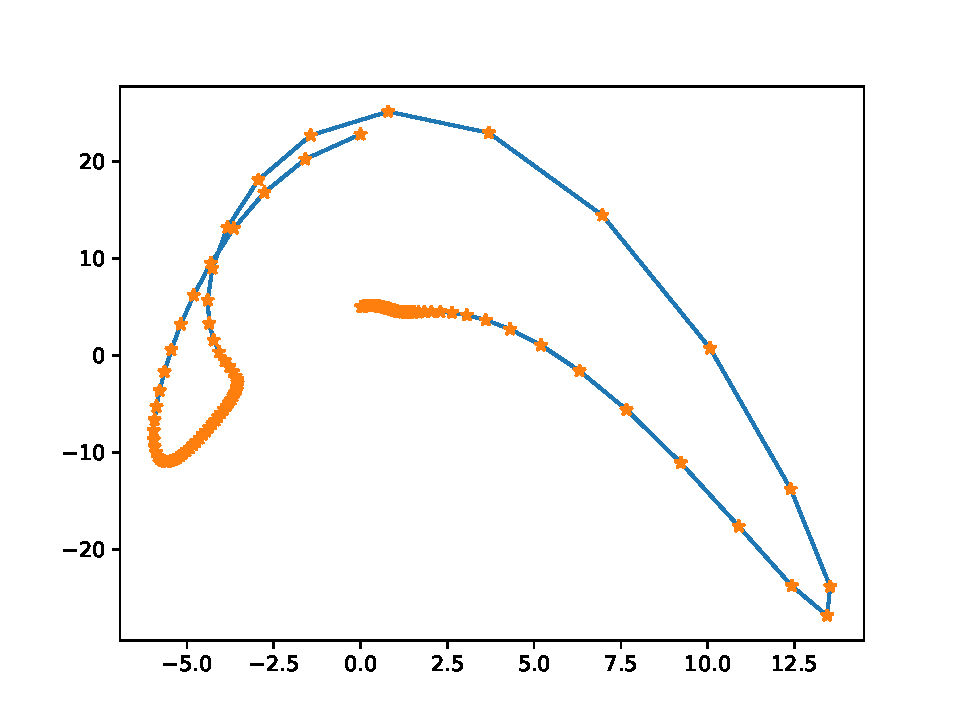
\includegraphics[width=\linewidth]{figures/curve_1/curve_q_pc.pdf}
        \caption{\(\bar q\)}
    \end{subfigure}
    \begin{subfigure}[t]{0.5\textwidth}\label{fig:curve_1_pc_r}
        \centering
        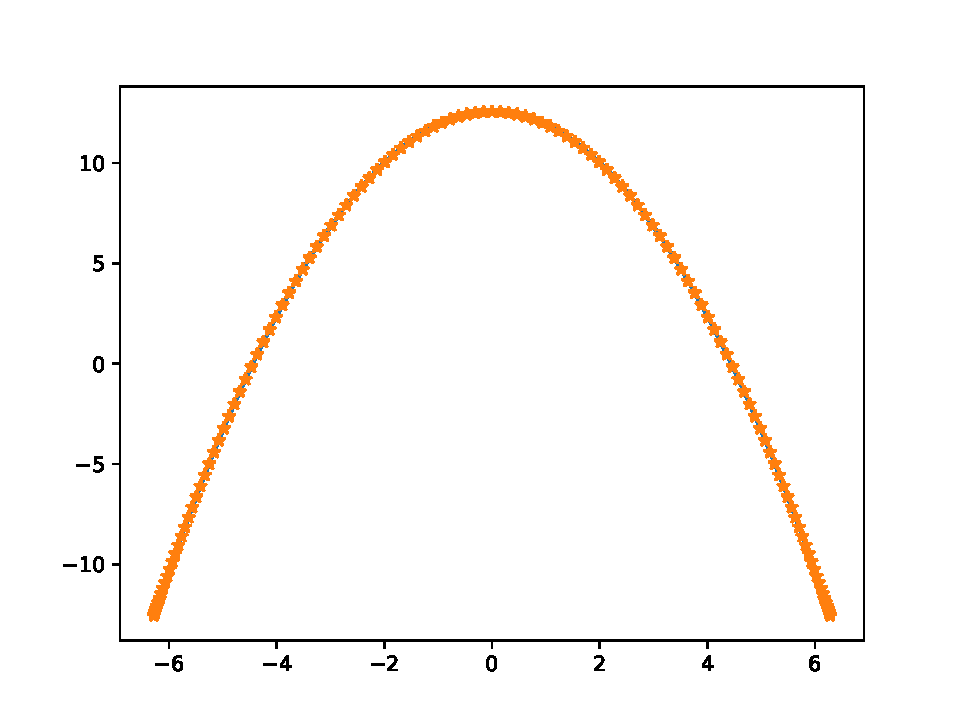
\includegraphics[width=\linewidth]{figures/curve_1/curve_r_pc.pdf}
        \caption{\(\bar r\)}
    \end{subfigure}
    \caption{The trajectory of \(\bar q\) and \(\bar r\) being piecewise constant interpolations of $q$ and $r$ from test problem (1).}
\end{figure}

\begin{figure}[t]\label{fig:curve_1_pc_pl_example}
    \begin{subfigure}[t]{0.5\textwidth}
        \centering
        \includegraphics[width=\linewidth]{figures/curve_1_pc/curve_pc_1/curve_pc_1_0_0.pdf}
        \caption{The approximate optimal reparametrization and the analytical solution.}
        \label{fig:curve_1_pc_solution}
    \end{subfigure}
    \begin{subfigure}[t]{0.5\textwidth}
        \centering
        \includegraphics[width=\linewidth]{figures/curve_1_pc/curve_pc_1/history_curve_pc_1_0.pdf}
        \caption{The cost function \(L(\theta)\) with each iteration.}
        \label{fig:curve_1_pc_history}
    \end{subfigure}
    \begin{subfigure}[t]{0.5\textwidth}
        \centering
        \includegraphics[width=\linewidth]{figures/curve_1_pl/curve_1_pl_exp_1/curve_1_pl_exp_1_1_0.pdf}
        \caption{The approximate optimal reparametrization and the analytical solution.}
        \label{fig:curve_1_pl_solution}
    \end{subfigure}
    \begin{subfigure}[t]{0.5\textwidth}
        \centering
        \includegraphics[width=\linewidth]{figures/curve_1_pl/curve_1_pl_exp_1/history_curve_1_pl_exp_1_1.pdf}
        \caption{The cost function \(L(\theta)\) with each iteration.}
        \label{fig:curve_1_pl_history}
    \end{subfigure}
    \caption{The approximate solutions to the piecewise constant (\ref{fig:curve_1_pc_solution}) and piecewise linear (\ref{fig:curve_1_pl_solution}) version of test problem (1). The approximate solution is compared to the analytical solution of test problem (1) and the corresponding training history is shown in the figure to the right.}
\end{figure}

\begin{figure}[t]\label{fig:curve_1_pl_eks}
    \begin{subfigure}[t]{0.5\textwidth}
        \centering
        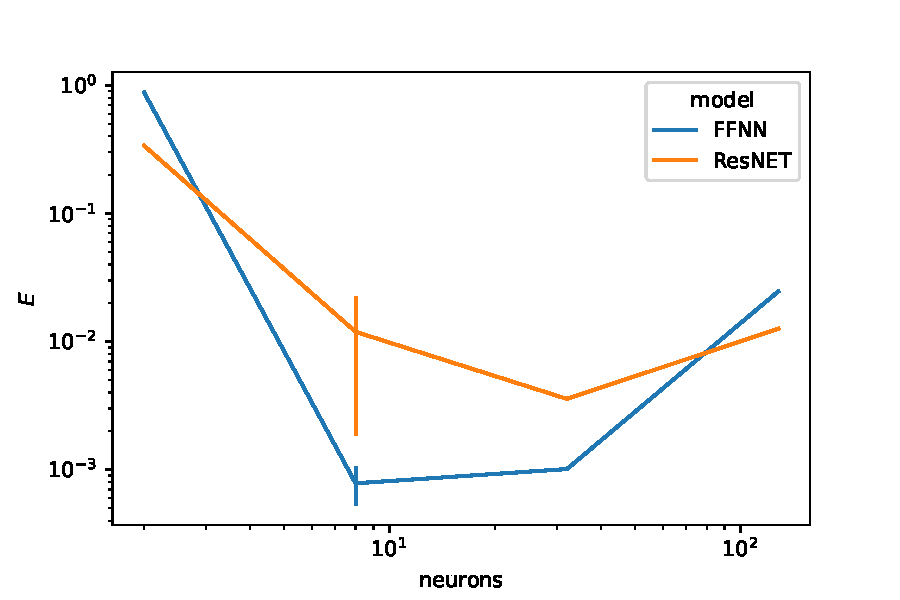
\includegraphics[width=\linewidth]{figures/curve_1_pl/curve_1_pl_exp_1/neurons_error.pdf}
        \caption{The final cost \(E\) with the number of neurons in each hidden layer.}
        \label{fig:curve_1_pl_neuron_error}
    \end{subfigure}
    \begin{subfigure}[t]{0.5\textwidth}
        \centering
        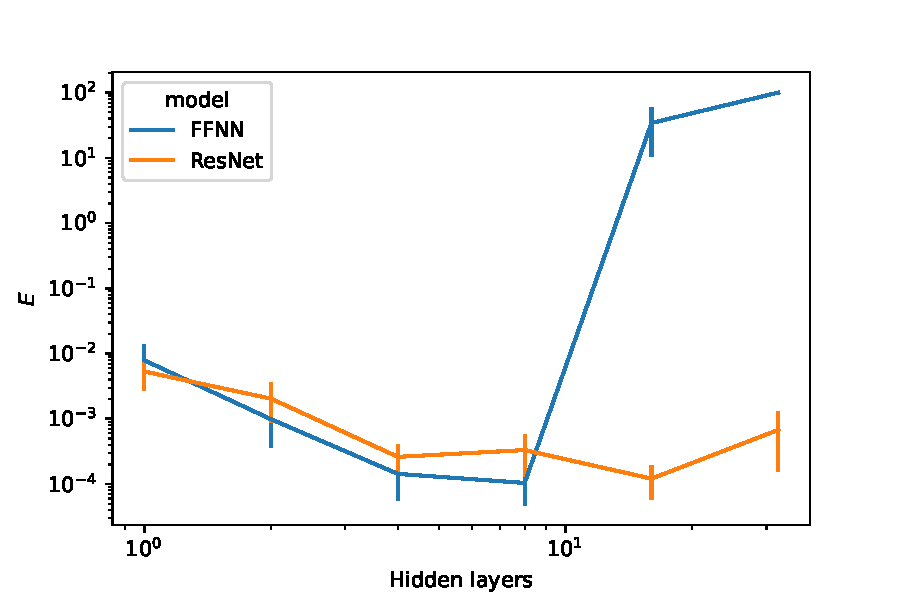
\includegraphics[width=\linewidth]{figures/curve_1_pl/curve_1_pl_exp_1/layer_error.pdf}
        \caption{Final cost \(E\) with the number of layers.}
        \label{fig:curve_1_pl_layer_error}
    \end{subfigure}
    \caption{Result of ensemble training for the piecewise linear version of test problem (1) with different number of neurons and hidden layers. In Figure \ref{fig:curve_2_neuron_error} the number of layers was fixed at 2. In Figure \ref{fig:curve_2_layer_error} the number of neurons is fixed at 8 per hidden layer. The error bars denote a 80\% confidence interval found by bootstrapping.}
\end{figure}

Training of